\section{Examples from Biology}
\label{sec:examples}
\subsection{Child Birth}
\label{subsec:examples-pregnancy}
\begin{frame}{\insertsubsection}
    \begin{figure}
        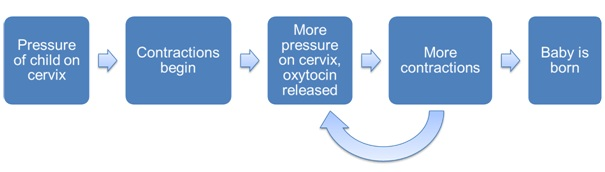
\includegraphics[width=\textwidth]{media/Childbirth.jpg}
        \caption{Childbirth~\cite{albert2022}}
    \end{figure}
    \begin{itemize}[<+->]
        \item More pressure 
        \item[ ] $\rightarrow$ More contractions
        \item This is a \emph{positive feedback loop}.
    \end{itemize}
\end{frame}
%
%
\subsection{Temperature Regulation}
\label{subsec:examples-temperature}
\begin{frame}{\insertsubsection}
    \begin{minipage}[t]{0.349\textwidth}
        \begin{itemize}[<+->]
            \item More Sweat
            \item[ ] $\rightarrow$ Less Temperature
            \item More ...
            \item[ ] $\rightarrow$ Less ...
            \item This is a \emph{negative feedback loop}.
        \end{itemize}
    \end{minipage}%
    \begin{minipage}[t]{0.649\textwidth}
        \begin{figure}
            \centering
            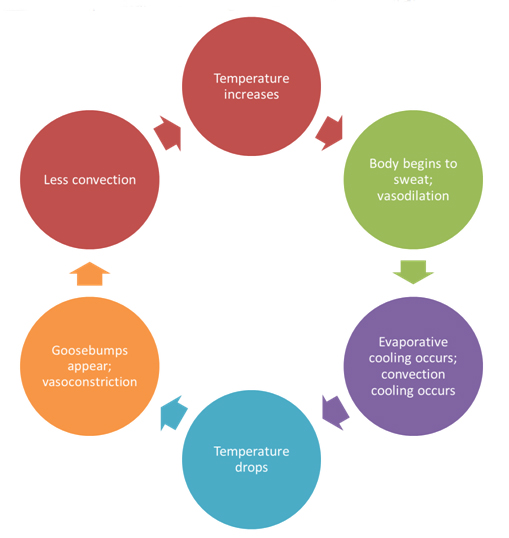
\includegraphics[width=\textwidth]{media/Temperature-Regulation.jpg}
            \caption{Temperature regulation~\cite{albert2022}}
        \end{figure}
    \end{minipage}%
\end{frame}
%
%
\subsection{More Examples}
\label{subsec:more-examples}
\begin{frame}{\insertsubsection}

    \begin{itemize}[<+->]
        \item Tight calcium regulation in humans
        \item Receptor Networks
        \item Synthetic Biology
        \item Optogenetics (What we also do)
        \item Financial Markets
        \item Social Relationships
        \item ...
    \end{itemize}
\end{frame}
%
%